\documentclass{assignment-263}


\anum{3}
\course{CSC263}
\duedate{March 30, 2022}
\filename{ps3soln.pdf, ps3soln.tex, csc263\_ps3.py }

\begin{document}

\think

\textbf{Please see the course syllabus for the late submission policy.}

\begin{enumerate}
\item[1.]  \textbf{[15 points]} Consider the following graph traversal algorithm,
    where instead of a queue \verb|Q|,
    we use a collection \verb|Col| that supports the operations:
    \begin{itemize}
        \item \verb|Add(Col, e)|: add an element to the collection
        \item \verb|IsEmpty(Col)|: returns whether the collection is empty
        \item \verb|ExtractRandom(col)|: returns a uniformly random element from the collection, and removes that element from the collection
    \end{itemize}

\begin{verbatim}
RandomTraversal(G=(V, E), s):
 1   for all v in V:
 2      colour[v] = white
 3   Col = Collection() # described above
 4   colour[s] = gray
 5   Add(Col, s)
 6   while not IsEmpty(Col):
 7       u = ExtractRandom(Col)
 8       for each neighbour v of u:
 9          if colour[v] = white
 10            colour[v] = gray
 11            Add(Col, v)
 12      Print(u)
 13      colour[u] = black
\end{verbatim}

\begin{enumerate}
\item (2 points)
We wish to call RandomTraversal on the graph $G$ with the edges
$$\{(A, B), (B, C), (C, D), (A, D), (A, E), (E, F)\}$$
Suppose we start at the vertex \verb|s=A|.
Is it possible to obtain the following output? Explain why or why not. 
\begin{verbatim}
A
B
C
D
E
F
\end{verbatim}
Yes, it is possible to obtain this output. For achieving such output, since A is the first Output, A is the starting vertex.\\
And when A entered, its neighbours B, D, E will be added to the \verb|Col|. \\
And after A has been printed, A become black, and we have to choose other element from the \verb|Col| by randomly, assume B has been selected, after B entered, the neighbour of B, which is C will be add to the \verb|Col|. And now C,D,E is in the Col.\\
Assume that C has been chose after B has been printed. After C entered, since the neighbour of C is D, and D is already is in the \verb|Col|, so nothing will be added to \verb|Col|. And now D, E is in the \verb|Col|.\\
Assume that D has been chose after C has been printed. After D entered, since the neighbour of D, which is A and C, the element C is already being black, and A is already in the \verb|Col|. So, nothing will be added to the \verb|Col|. and now only E is in the \verb|Col|.\\
After D has been printed, E will entered, the neighbour of E will be added to the \verb|Col|, which is F. And after E being printed, only F left, so the last element to print is F.\\
As a result, it is possible to obtain this output.
\item (2 points)
Suppose we call \verb|RandomTraversal| on the graph $G$ from part (a).
Is it possible to obtain the following output? Explain why or why not. 
\begin{verbatim}
A
F
E
B
C
D
\end{verbatim}
No, it is impossible to obtain such an output.\\
Since the first output is A, we must choose A as root.And when A entered, its neighbours B, D, E will be added to the \verb|Col|. \\
The second output is F, however, there is no such a element in the \verb|Col| after A enters.\\
As a result, it is impossible to achieve such an output.


\item (3 points)
Suppose we call \verb|RandomTraversal| on the graph $G$ from part (a).\\
I use a tree graph for this question, the graph can be seen in the last page.\\
Thus, the probability is $\frac{1}{3}$ $\times$ ( $\frac{1}{3}$ $\times$ $\frac{1}{2}$ $\times$ $\frac{1}{2}$ + $\frac{1}{3}$ $\times$ $\frac{1}{3}$ + $\frac{1}{3}$ $\times$ $\frac{1}{3}$ $\times$ $\frac{1}{2}$) + $\frac{1}{3}$ $\times$ ($\frac{1}{2}$ $\times$ $\frac{1}{2}$ $\times$ $\frac{1}{2}$ + $\frac{1}{2}$ $\times$ $\frac{1}{2}$ $\times$ $\frac{1}{2}$ + $\frac{1}{2}$ $\times$ $\frac{1}{2}$) +  $\frac{1}{3}$ $\times$  ( $\frac{1}{3}$ $\times$  $\frac{1}{3}$ $\times$ $\frac{1}{2}$ + $\frac{1}{3}$ $\times$  $\frac{1}{3}$ + $\frac{1}{3}$ $\times$ $\frac{1}{2}$ $\times$ $\frac{1}{2}$ + $\frac{1}{3}$ $\times$ $\frac{1}{2}$ + $\frac{1}{3}$) = $\frac{4}{9}$

\item (4 points)
Suppose our collection \verb|Col| stores its elements in a linked list,
and has a counter $n$ that tracks the number of elements in the linked list. Moreover,
suppose that \verb|Col| is a data structure with the following supported operations:

\begin{itemize}
    \item \verb|Add(x)| inserts a new element $x$ to the head of the linked list, and increments $n$
    \item \verb|IsEmpty()| checks whether $n$ is 0.
    \item \verb|ExtractRandom()| chooses a random number $i$ between 1 and $n$ (an operation with constant cost), and returns and deletes the $i$th element of the linked list.
\end{itemize}

What is the worst-case runtime of RandomTraversal, in terms of $|V|$ and $|E|$?
Provide a $\Theta$ bound, and explain how you obtained the result.
(Note: we are no longer just considering the graph $G$ from the earlier parts of this question.)\\\\
Since the Col is a linkedlist, by the definition of linkedlist, function Add is O(1), and ExtractRandom() is O(n) in linkedlist.\\
In the function RandomTraversal, from line 1 to 2, it runs a for loop, and each step, which is line 2 is a  O(1) function, so the total runtime from line 1 to 2 is $|V|$. from line 6 to line 7, the function run a ExtractRandom() for each vertex, and a single ExtractRandom is O(n), and in this case, n = $|V|$, so the total runtime from 6 to 7 is $|V|^2$. And from line 8 to 11, the function check each neighbour for all vertex, which is check all the edge, so the run time for this step is $|E|$.
Thus, the total runtime = $|V|^2$ + $|E|$ + $|V|$, which is $O$($|V|^2$ + $|E|$)

\item (4 points)
Provide another implementation of the data structure \verb|Col| so that the cost of RandomTraversal 
becomes $O(|V|+|E|)$. Briefly justify that your approach is correct, and has the desired runtime.\\\\
In the 1(d), i noticed that the cause for runtime getting $O$($|V|^2$ + $|E|$) is because of the runtime for each ExtractRandom is $O$($|V|$); thus, to achieving $O(|V|+|E|)$, i have to use a data-structure has $O$(1) for ExtractRandom() as \verb|Col|; and i pick dictionary as its data structure.\\
Since the ExtractRandom for dictionary is $O$(1) by the definition in python, when running a RandomTraversal.  from line 1 to 2, it runs a for loop, and each step, which is line 2 is a  O(1) function, so the total runtime from line 1 to 2 is $|V|$. from line 6 to line 7, the function run a ExtractRandom() for each vertex, and a single ExtractRandom is O(1), so the total runtime from 6 to 7 is $|V|$. And from line 8 to 11, the function check each neighbour for all vertex, which is check all the edge, so the run time for this step is $|E|$.
Thus, the total runtime = $|V|$ + $|E|$ + $|V|$, which is $O$($|V|$ + $|E|$)

\end{enumerate}

\item[2.]  \textbf{[10 points]} 
    You dream that you were somehow enrolled in a course called ``The Philosophy of Logical Paradoxes",
    and the final exam is happening... now! You didn't study for the exam, but luckily
    the entire exam question is a series of $N$ statements that you must label \verb|True| or \verb|False|.
    Each statement is of the form \verb|Statement X is TRUE/FALSE|, where $X$ is between 1 and $N$.
    Here is one example of such a set statements (with $N=2$):

	\begin{verbatim}
		    1. Statement 2 is FALSE.
		    2. Statement 1 is TRUE.
	\end{verbatim}

    In this above example, there is a \textbf{paradox}: a group of statements that lead to a contradiction.
	If we assume Statement 1 is True, then Statement 2 is False, which
	in turn means Statement 1 is False. But if we assume Statement 1 is
	False, then Statement 2 is True, which in turn means Statement 1
	is True. So Statement 1 is True iff Statement 1 is False, a blatant
	contradiction.

    In your dream, you remember that you learned about graphs in CSC263.
    You can thus devise an algorithm to determine whether the group of statements in the exam
    forms a paradox, thus allowing you to waking you up from the dream.

    %Your task is to figure out whether this group of statements forms a paradox.
	In particular, answer the following questions.
	\begin{enumerate}%[label=(\alph*),topsep=\parsep]

    \item (2 points)
		Describe how to construct a graph to solve this problem. Be
		precise: state clearly what vertices your graph contains (and what
		each vertex represents) and what edges your graph contains (and what
		each edge represents).\\\\
	The graph will have 2N vertices and 2N edges, which N will represented the number of statements in the test, the vertices will be 1True, 1False, 2True, 2False, ..., NTrue and NFalse.\\
	Vertices: each vertice will represented by two attributes, the first attribute is a integer, which represent the statement it belongs to, and the second attribute is a boolean, which represent this vertex is true or false. Since there are N statement in the test, so the graph will have 2N vertices, which N of them represent the true statements, and the others represent the false statements.\\
	Edges: Each edge will represent the relationship between each statements, for example, if statement 1 is Statement 2 is FALSE; then there will be two edges, one of edges is connect by 1True and 2False, the other one will be 1False and 2True. since there are N statements, and each statement could have a negate version if the statement itself is false, so there will be 2N edges totally.

	\item (2 points)
		Give a necessary and sufficient condition for the $N$
		statements to form a paradox. Justify your answer.\\\\
	I think the necessary and sufficient condition for the $N$ statements to form a paradox is there is a path from xTrue to xFalse in the graph, where x is a statement and belongs to $N$.\\
	Proof for sufficient: if there is a path from xT to xF in the graph, prove that there is a paradox.\\
	Since there is a path from xTrue to xFalse, if statement x is True, then statement x is False by the statement x, and this is a paradox by the definition. Thus, this is a sufficient condition.\\
	Proof for necessary: Assume there is such a paradox exist that there is a paradox, but there is no path from yTrue to yFalse such that y $\in$ $N$.\\
	Since the paradox exist, there must be a statement in the paradox exist that would cause a contradiction. So that there must exsist a path from zTrue to zFalse such that z $\in$ $N$, which is contridict with the assuming.\\
	Thus, This is a necessary condition.

	\item (3 points) How do you efficiently detect whether your graph from
        part (a) satisfies your condition described in
        part (b)? Describe your algorithm in concise (but
		precise) English.
	I will choose DFS for this question.\\\\
	Firstly, i will run the whole graph by using DFS, and letting statement 1True as its root.\\
	After run the whole graph by DFS, i will check whether xTrue is the ancestor or descendant of xFalse,for any x $\in$ $N$. By checking the ancestor or descendant, i will check it by using the start and finish time; if xTrue's start time is less that xFalse's start time, and xTrue's finish time is greater than xFalse's finish time, that means xTrue is the ancestor of xFalse. And if xTrue's start time is greater that xFalse's start time, and xTrue's finish time is less than xFalse's finish time, that means xTrue is the descendant of xFalse.\\
	And if any xTrue is the ancestor or descendant of xFalse for x $\in$ $N$, that means that there is a paradox; otherwise, if none of xTrue is the ancestor or descendant of xFalse, that means there is no paradox exists.
	
    \item (3 points) Show that the worst-case runtime of your algorithm is $\Theta(N)$.\\\\
    Firstly, the worst-case's runtime for a DFS is equals to $|V|+|E|$ = 2N + 2N = 4N \\
    And for when we check each statement, we only need to check whether the true and false vertex's start time and finish time is satisfy the condition; which is mentions in the part c, and this could be done by a simple logic if-statement, so the runtime for checking 1 statement is 1, and we need to check all statement, so the total time for checking is N.\\
    Thus, the total time for the worst-case runtime of my algorithm is  4N + N = 5N, which is is $\Theta(N)$.
	\end{enumerate}

\item[3.]  \textbf{[5 points]} 
    Let $G = (V, E)$ be a connected undirected graph. Suppose we run BFS on this graph starting
    from some vertex $s \in V$. Recall that we showed that the subset of edges
    $T = \{(\pi[v], v) \in V\}$ forms a spanning tree of $G$.

    Suppose we assign a weight $w(e)$ to each edge $e = {u, v} \in E$, with 
    $w(e) = d[u] + d[v]$, where $d[u]$ and $d[v]$ are values computed during BFS. Prove or disprove that $T$ is
    a minimum spanning tree. \\\\
    T is the minimum spanning tree.\\
    Provement:\\
    Assume there is such a tree T' exist, $\sum$ $w(e)$ in T' $<$ $\sum$ $w(e)$ in tree provided by BFS.\\
    Then, $\exists$ an edge e' in T' that $w(e')$ $<$ $w(e)$.\\
    By the definition of MST Kruskal Algorithm; each edge should be the smallest edge in the graph.\\
    Since the graph is run by a BFS, when the tree is a MST, each edge should only be tree edges, which is suppose to be level by level.
    thus, min($w(e)$) = d[u] + d[v], and there is no such a e' exist that $w(e')$ $<$ $w(e)$, which cause a contradiction.\\
    So, T' is not exist, in conclusion, T is the minimum spainning tree.
    

\program

\item[4.] \textbf{[5 points]} You wake up from the dream you had
    back in Question 2, and realize that your CSC263 Problem Set 3
    actually asks you to write a program to solve this exact problem!
    What a coincidence!

    Complete the function \verb|detect_paradox| that takes a list of $N$ statements.
    Each statement is of the form \verb|Statement X is TRUE/FALSE|,
    where $X$ is between 1 and $N$.

    Your function should return a list containing the \textit{subset of statements that are incompatible with each other},
    or the empty set if there is no paradox. Here are some examples

    \begin{verbatim}
    >>> detect_paradox(['Statement 2 is FALSE',
                        'Statement 1 is TRUE',
                        'Statement 3 is TRUE'])
    [1, 2]
    >>> detect_paradox(['Statement 2 is FALSE',
                        'Statement 1 is TRUE',
                        'Statement 3 is FALSE'])
    [1, 2, 3]
    >>> detect_paradox(['Statement 3 is FALSE',
                        'Statement 3 is FALSE',
                        'Statement 4 is FALSE',
                        'Statement 4 is TRUE'])
    [] # there is no paradox
    \end{verbatim}

    The order of the elements in your list does not matter. In other words, in the first example,
    you can return the list \verb|[2, 1]| instead of the list \verb|[1, 2]|, and both answers
    will be considered correct.

\textbf{Requirements}:
\begin{itemize}
\item Your code must be written in Python 3, and the filename must be \verb|csc263_ps3.py|.
\item We will grade only the \verb|detect_paradox| function;
      please do not change its signature in the starter code.
      Include as many helper functions as you wish.
\item All code that you submit must be your own, including any helper functions.
\item Your code must compile and otherwise be testable in order to earn credit
      for the auto-graded portion of this question.
\item For each test-case that your code is tested on, your code must run within
10x the time taken by our solution. Otherwise, your code will be considered to have timed out.
\item You do not need to include a written part for this question, since you have already done so in Q2.
\end{itemize}

\end{enumerate}
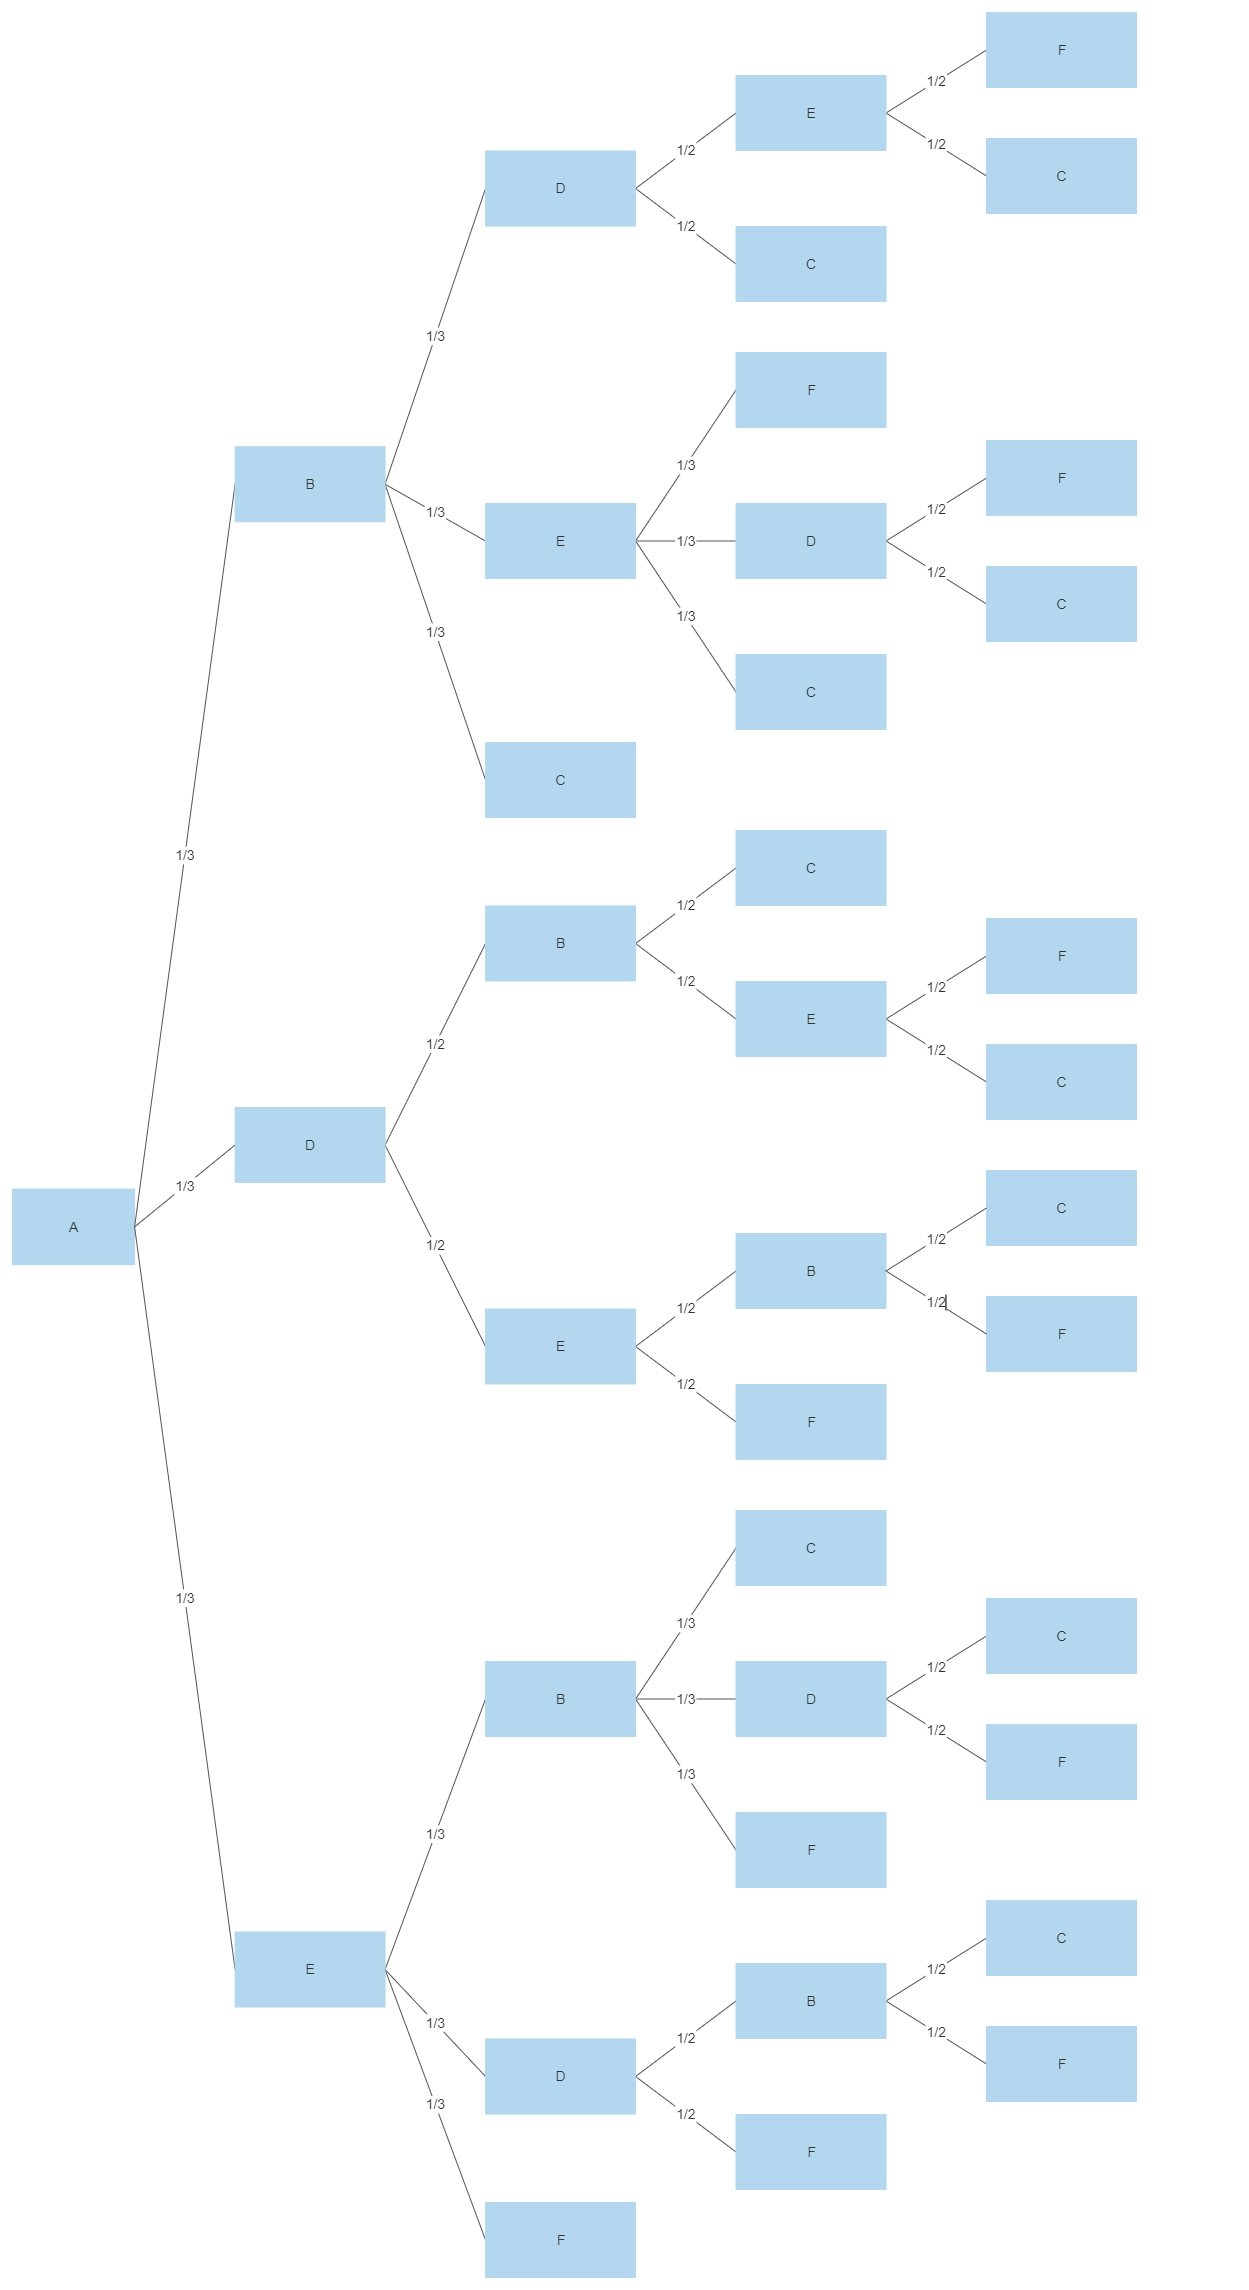
\includegraphics[width=1\textwidth, inner]{Decision_Tree.jpg}
\end{document}

%%% Local Variables:
%%% mode: latex
%%% TeX-master: t
%%% End:
